% -*- coding: utf-8 -*-
%\documentclass{article}
\documentclass{ctexart}

\usepackage{CJK}
\usepackage{geometry}
\usepackage{upgreek}
\usepackage{amsmath}
\usepackage{indentfirst}
\usepackage{geometry}
\usepackage{upgreek}
\usepackage{fancybox}
\usepackage{indentfirst}
\usepackage{url}
\usepackage{graphicx}
\usepackage{listings}
\usepackage{fancyhdr}

\author{Your Name}

\title{Test Document}

\begin{document}
\begin{CJK*}{GBK}{song}


\maketitle

\section{sec1}
This is a test document
\subsection{sec2}
This is a test document2
\subsubsection{sec3}
This is a test document3
\paragraph{paragraph}
xxxx


\begin{Sbox}
\begin{minipage}{\textwidth}
\begin{verbatim}
the --replicate-* options, can be set only when the slave server starts.
\end{verbatim}
\end{minipage}
\end{Sbox}
\fbox{\TheSbox}

\parbox{17em}{There are two ways to incorporate images into your LaTeX document, and both use the graphicx package by means of putting the command \textbackslash usepackage\{graphicx\} near the top of the LaTeX file, just after the documentclass command.}

\begin{itemize}
\item First thing
\item Second thing
\item Third thing
\end{itemize}

\begin{enumerate}
\item First numbered thing
\item Second numbered thing
\item Third numbered thing
\end{enumerate}

\begin{quote}
There are two ways to incorporate images into your LaTeX document, and both use the graphicx package by means of putting the command \textbackslash usepackage\{graphicx\} near the top of the LaTeX file, just after the documentclass command.
\end{quote}

\begin{description}
\item[First item] text
\item[Second item] dfe df
\item[Third item] dfexxdf
\item[4th item] sxe
\end{description}

\makebox[\textwidth]{\hrulefill}
\begin{verbatim}
#include <iostream>
using namespace std;
int main()
{
    cout<<"hello world"<<endl;
}
\end{verbatim}
\makebox[\textwidth]{\hrulefill}
\begin{verbatim}
from GChartWrapper import Pie
from GChartWrapper import Pie3D

p=Pie3D( [1,2,3,4] ).label('A','B','C','D').color('00dd00')
p.save('a.png')

p=Pie([5,10,15]).title('Hello Pie').color('red','lime').label('hello', 'world','Hello World')
p.save('b.png')
\end{verbatim}
\makebox[\textwidth]{\hrulefill}


\begin{table}[hbtp]
\caption{This table is an example}
\begin{center}
\begin{tabular}{c|c|c}
First row, first column & First row second column & First row, third column \\ \hline
Second row, first column & Second row, second column & Second row, third column \\
Third row, first column & Third row, second column & Third row, third column \\
\multicolumn{3}{c}{78}
\end{tabular}
\end{center}
\label{exampletable}
\end{table}



\begin{figure}[hbtp]
\caption{Img B}
\begin{center}
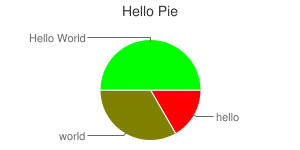
\includegraphics[scale=0.75]{b.png}
\end{center}
\label{fig1}
\end{figure}

\begin{tabular}{l*{6}{c}r}
Team              & P & W & D & L & F  & A & Pts \\
\hline
Manchester United & 6 & 4 & 0 & 2 & 10 & 5 & 12  \\
Celtic            & 6 & 3 & 0 & 3 &  8 & 9 &  9  \\
Benfica           & 6 & 2 & 1 & 3 &  7 & 8 &  7  \\
FC Copenhagen     & 6 & 2 & 1 & 2 &  5 & 8 &  7  \\
\end{tabular}


\begin{tabular}{| p{5cm} | c |}
        \hline
        \begin{verbatim}
        code
        \end{verbatim}
        & description
        \\ \hline
\end{tabular}

\begin{lstlisting}[frame=trBL]
from GChartWrapper import Pie
from GChartWrapper import Pie3D
p=Pie3D( [1,2,3,4] ).label('A','B','C','D')
                    .color('00dd00')
p.save('a.png')
p=Pie([5,10,15]).title('Hello Pie')
    .color('red','lime')
    .label('hello', 'world','Hello World')
p.save('b.png')
\end{lstlisting}

\end{CJK*}
\end{document} 